TicText is an iOS application built with Apple's Cocoa Touch framework, Facebook's Parse framework, and many other modules provided through CocoaPods (a dependency manager). The application, when joined with these frameworks, compose our entire infrastructure from front end to back end.

In the front end, the Cocoa Touch framework provides us with many inherent design patterns, such as Model-View-Controller and Chain of Responsibility for touch input, that trivialize most device interactions and let us focus on the application. The Parse framework enables our models to easily implement the Active Record pattern and provides out-of-the-box data caching.

In the back end, the Parse framework eliminates the tedious work of designing a schema and setting up an Apple push notification server. Hence, the entirety of our back end code is composed of triggers and stored procedures written in JavaScript.

%\begin{enumerate}
%	\item Include multiple UML diagrams to show the important parts of your system (you must have UML diagrams).
%	\item Describe in a top-down manner the architecture of your system.
%	\item Include enough details about the design of your system such that anyone who refers to your documentation can %understand the major components of your system and how they are related.
%	\item Describe how the choice of the framework influence the design of your system.
%\end{enumerate}

\noindent When a user uses TicText, they will interact with several major workflows:
\begin{enumerate}
	\item Onboarding (Sign up/Log in through Facebook + Find Friends)
	\item Setting the expiration time for a Tic
%	\item Viewing conversations and new Tics
%	\item Viewing a single conversation
	\item Composing a new Tic
%	\item Receiving a new Tic
\end{enumerate}

\renewcommand\listfigurename{List of Diagrams}
\listoffigures

\subsection{Expiration Picker}
\begin{figure}[H]
    \centering
    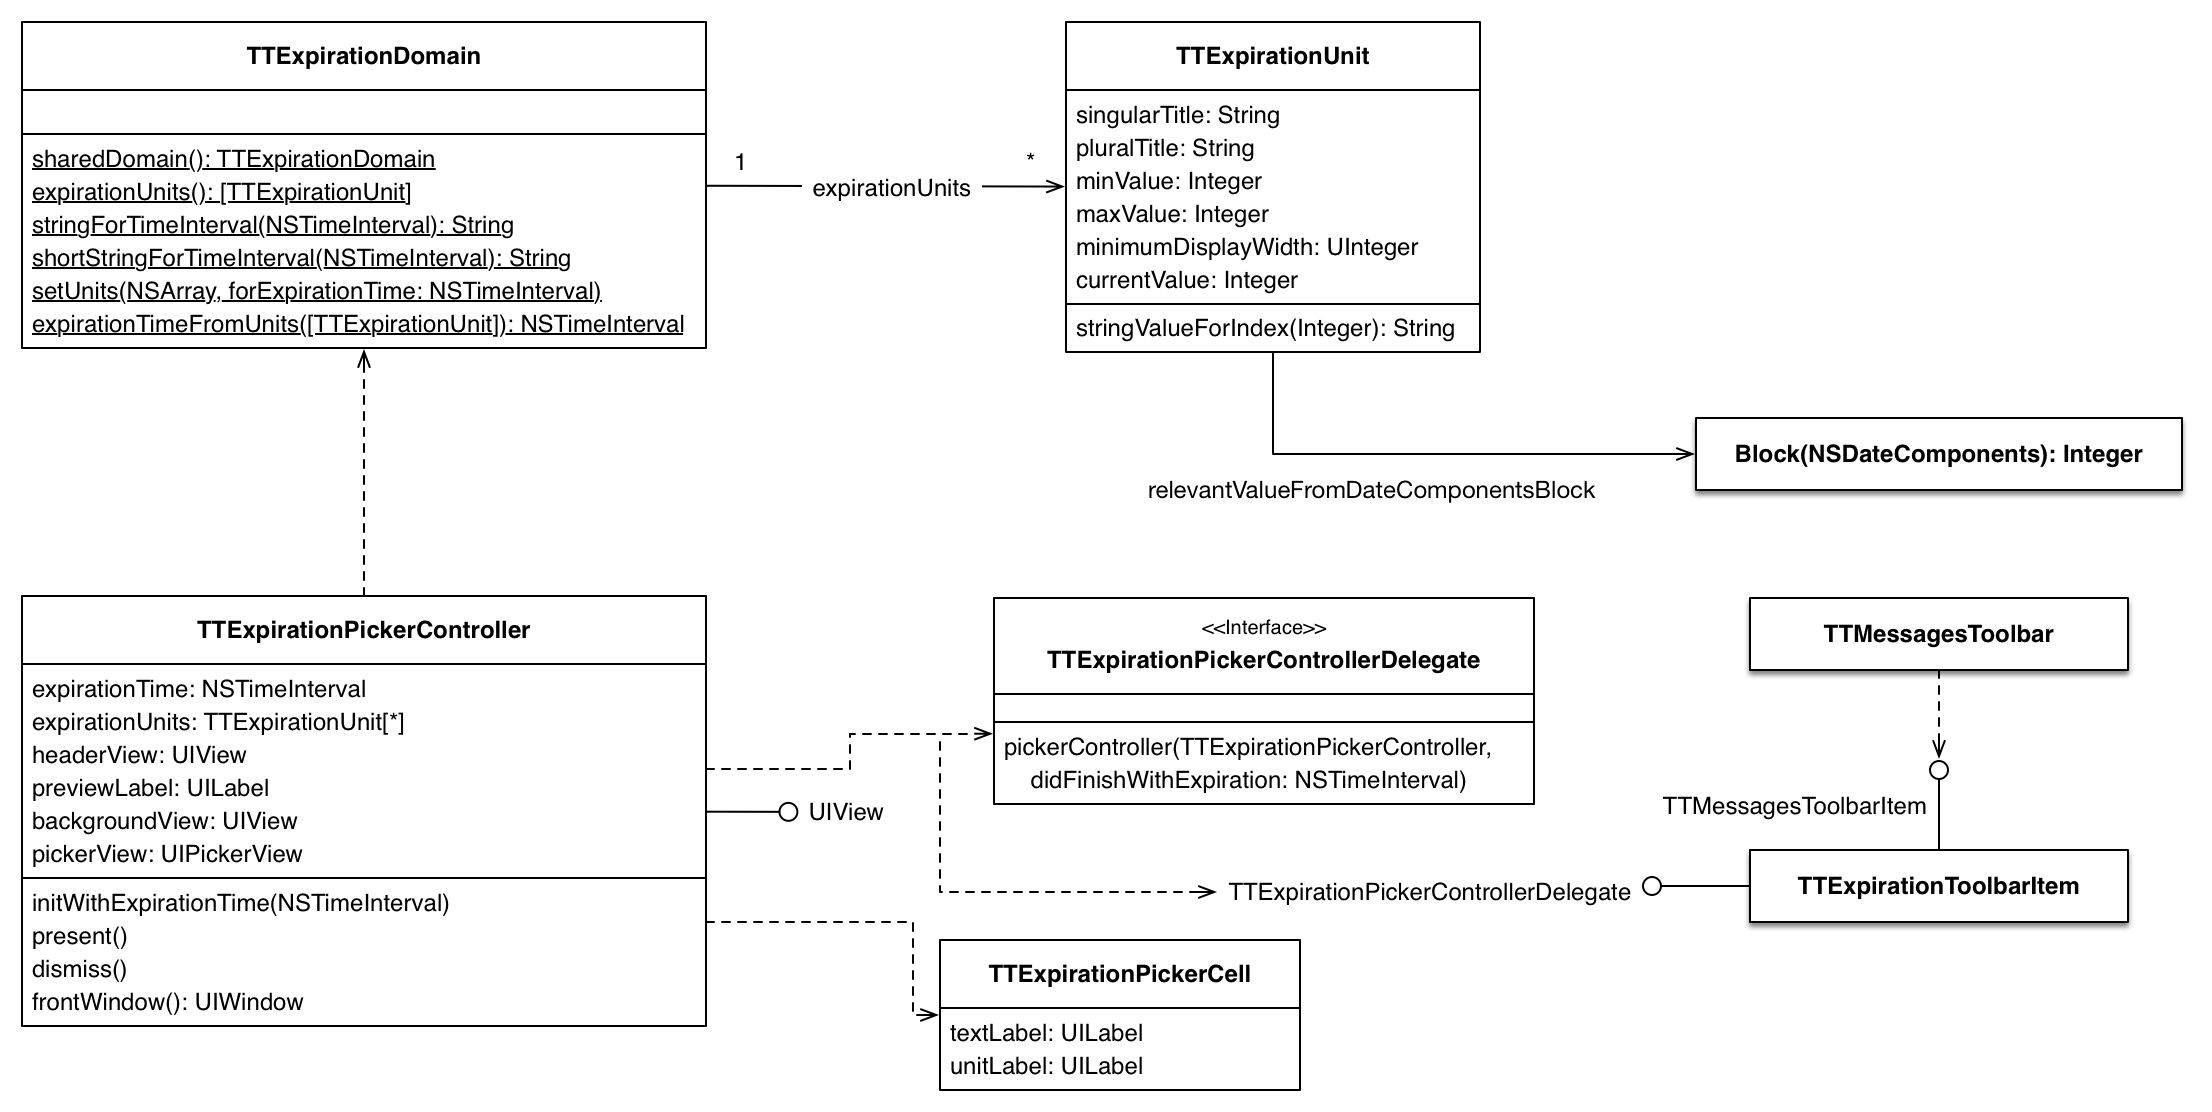
\includegraphics[width=\textwidth]{expirationpicker_class}
    \caption{Expiration Picker Class Diagram}
    \label{fig:expirationpicker_classdiagram}
\end{figure}

\begin{figure}[H]
    \centering
    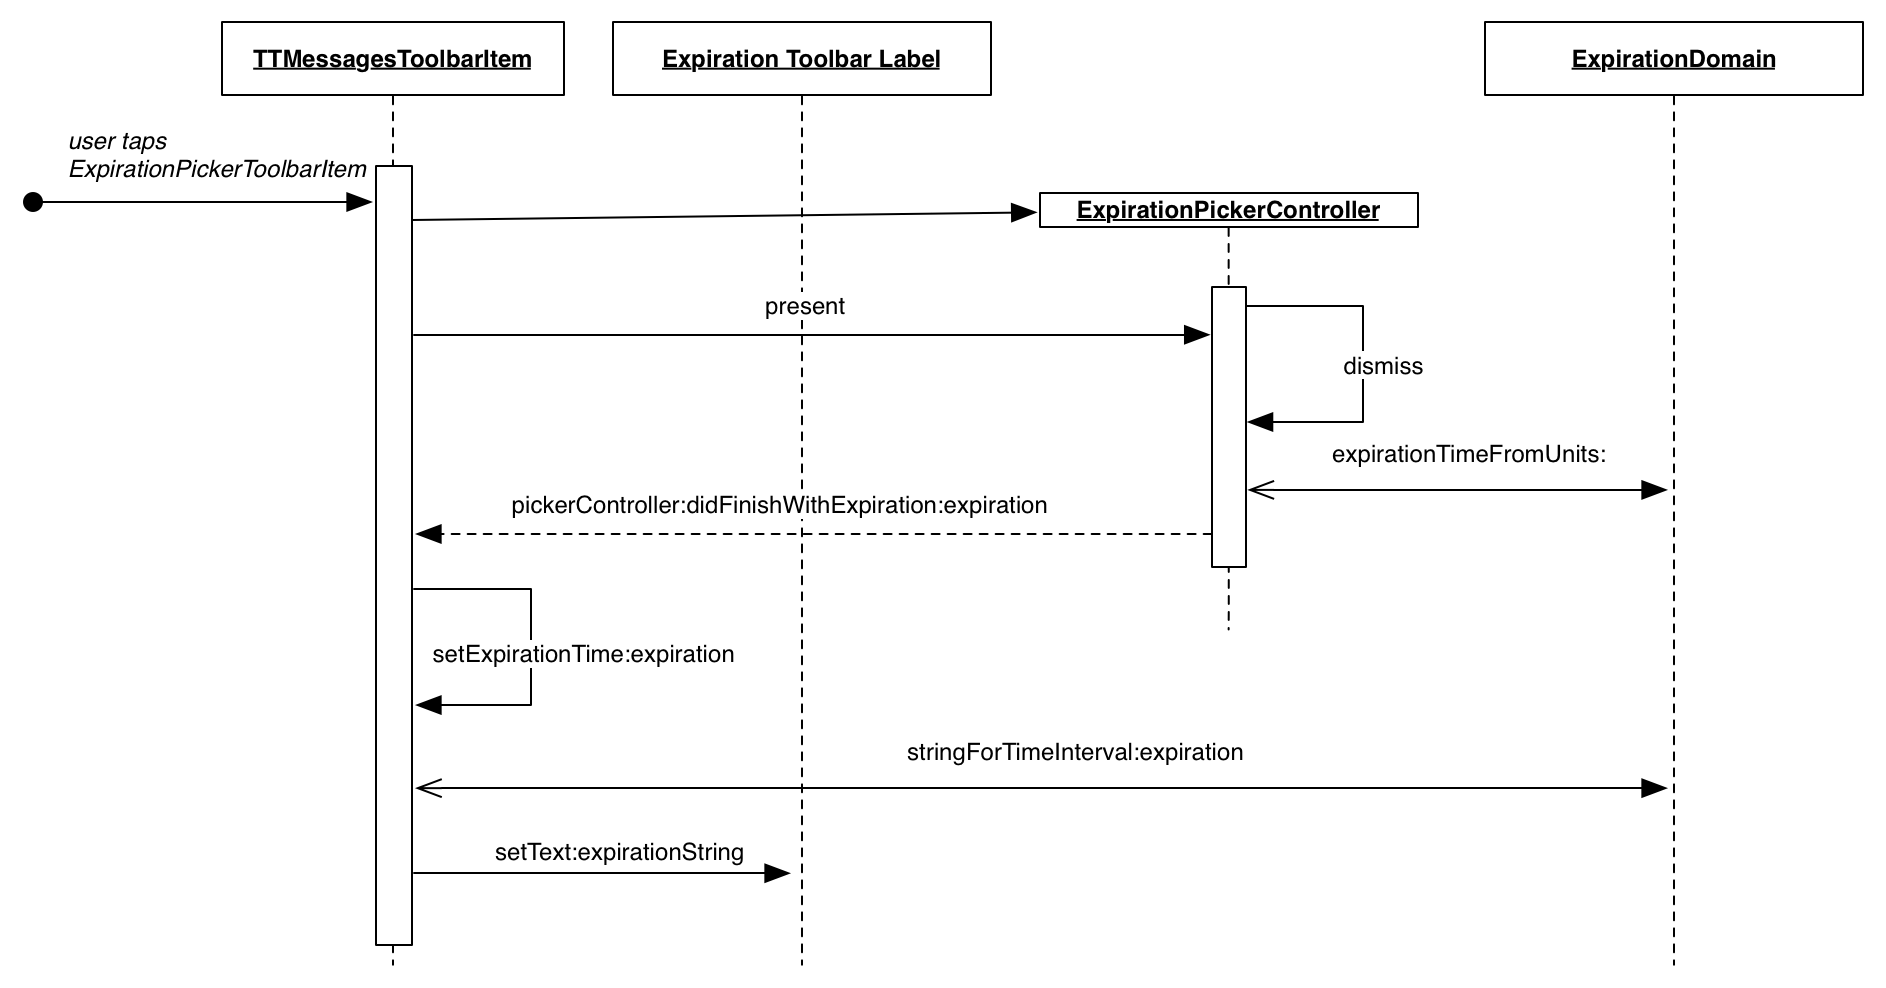
\includegraphics[width=\textwidth]{expirationpicker_sequence}
    \caption{Expiration Picker Sequence Diagram}
    \label{fig:expirationpicker_sequence}
\end{figure}

\begin{figure}[H]
    \centering
    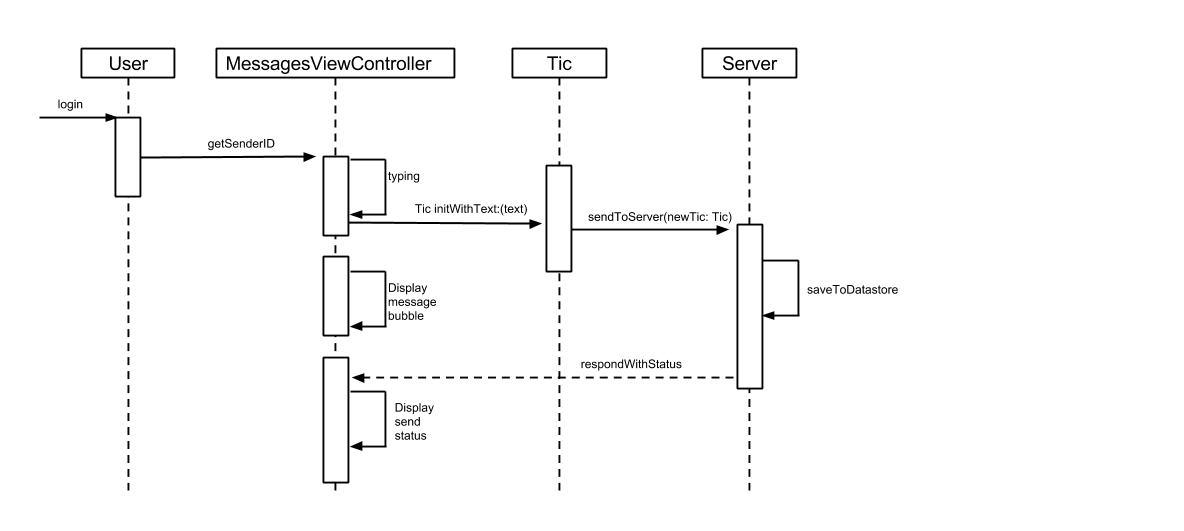
\includegraphics[width=\textwidth]{us11_sequence}
    \caption{Sending a Tic Sequence Diagram}
    \label{fig:us11_sequence}
\end{figure}

%\subsection{Sequence Diagrams}
%\begin{figure}[H]
%    \centering
%    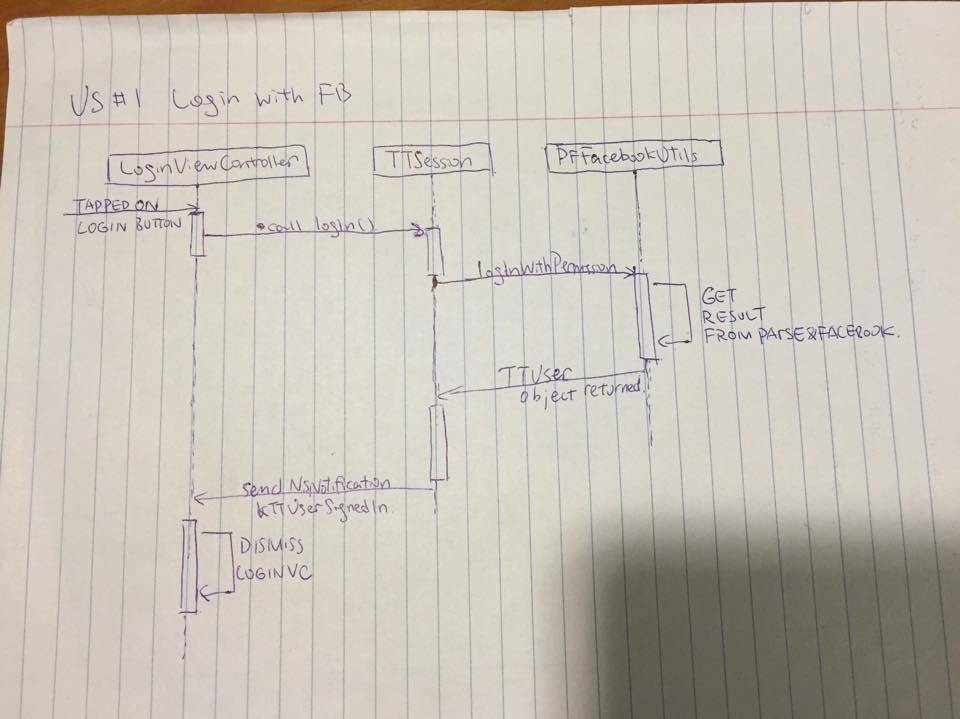
\includegraphics[width=0.8\textwidth]{us1_sequence}
%    \caption{US1 Sequence Diagram}
%    \label{fig:us1_sequence}
%\end{figure}

%\begin{figure}[H]
%    \centering
%    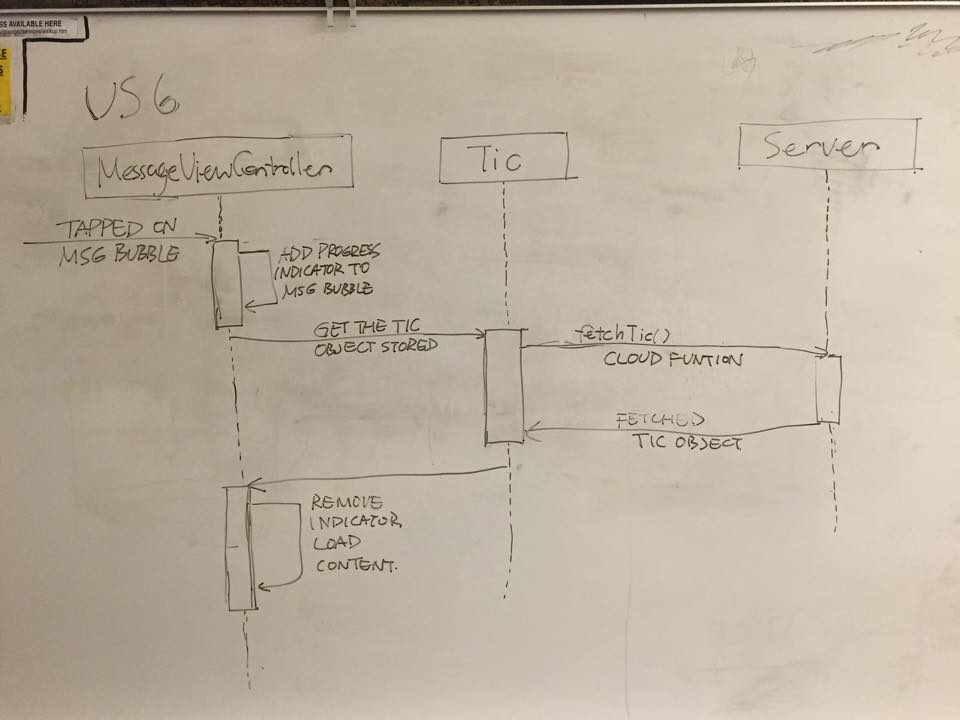
\includegraphics[width=0.8\textwidth]{us6_sequence}
%    \caption{US6 Sequence Diagram}
%    \label{fig:us6_sequence}
%\end{figure}

%\begin{figure}[H]
%    \centering
%    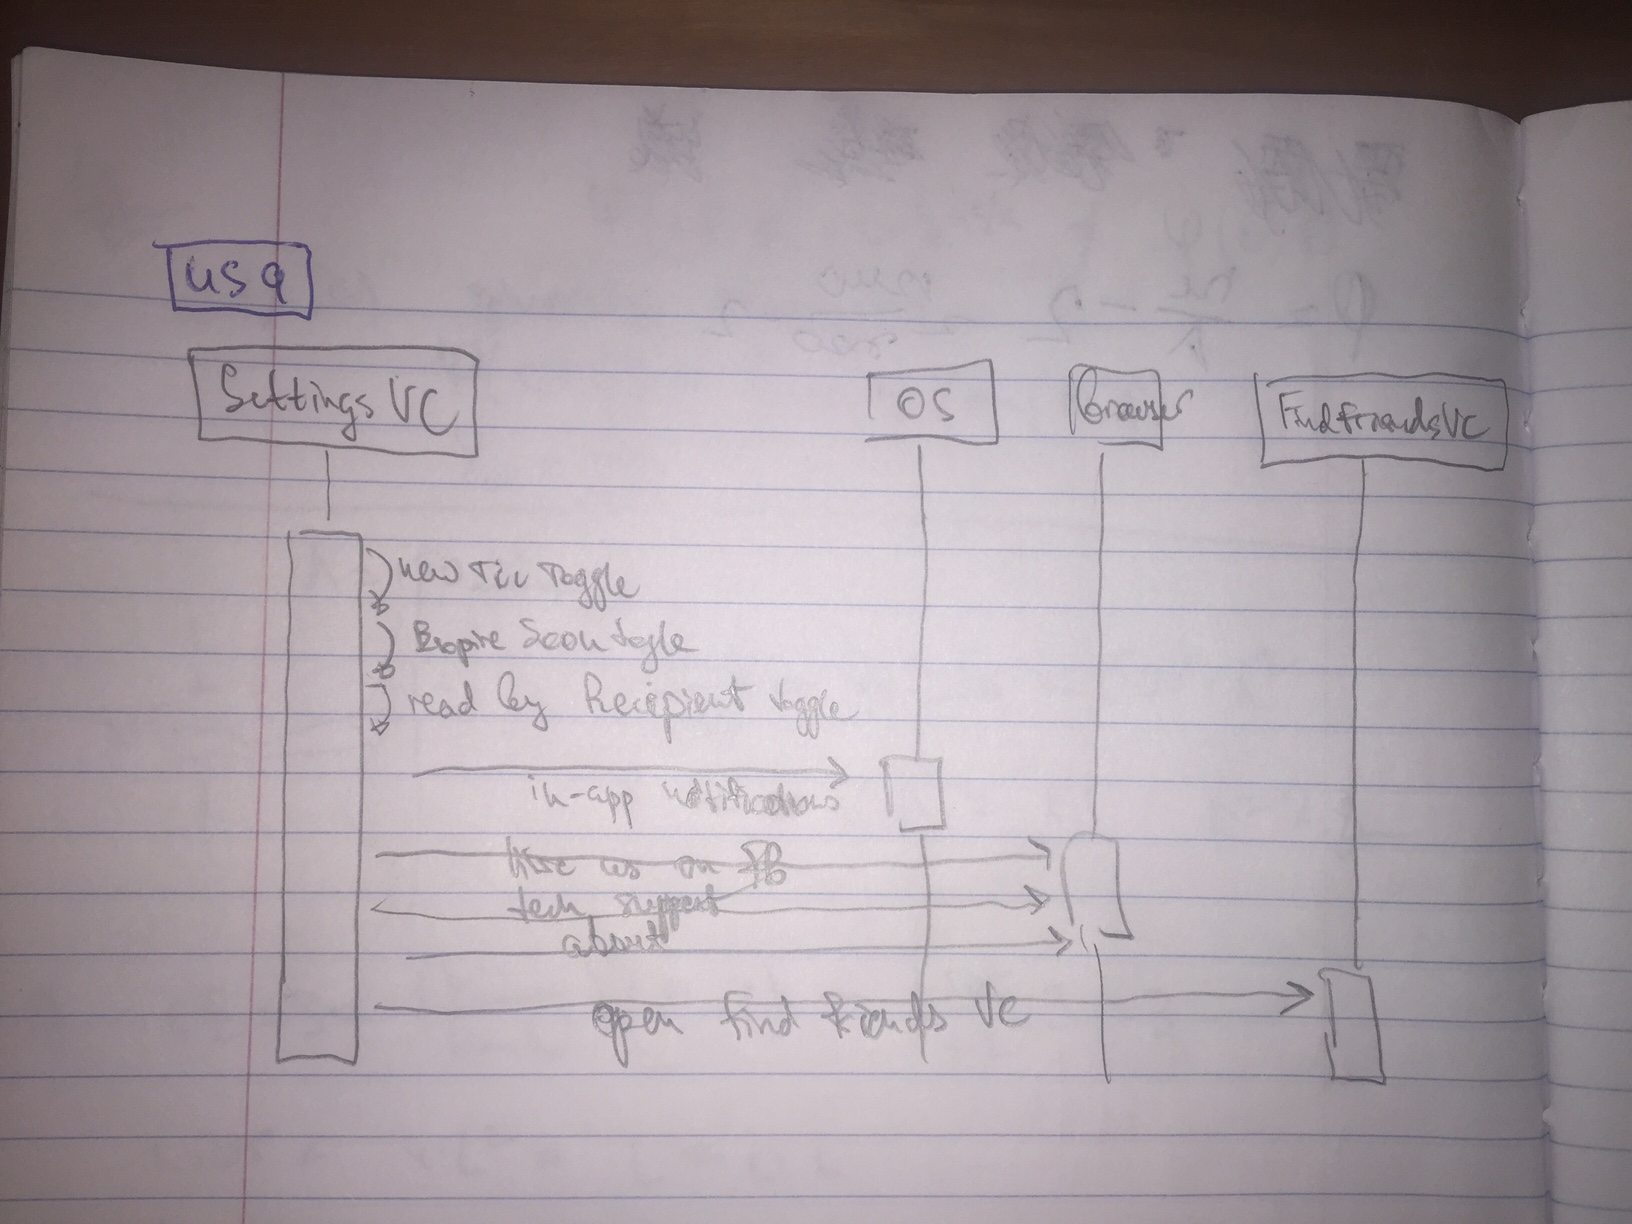
\includegraphics[width=0.8\textwidth]{us9_sequence}
%    \caption{US9 Sequence Diagram}
%    \label{fig:us9_sequence}
%\end{figure}

\begin{figure}[H]
    \centering
    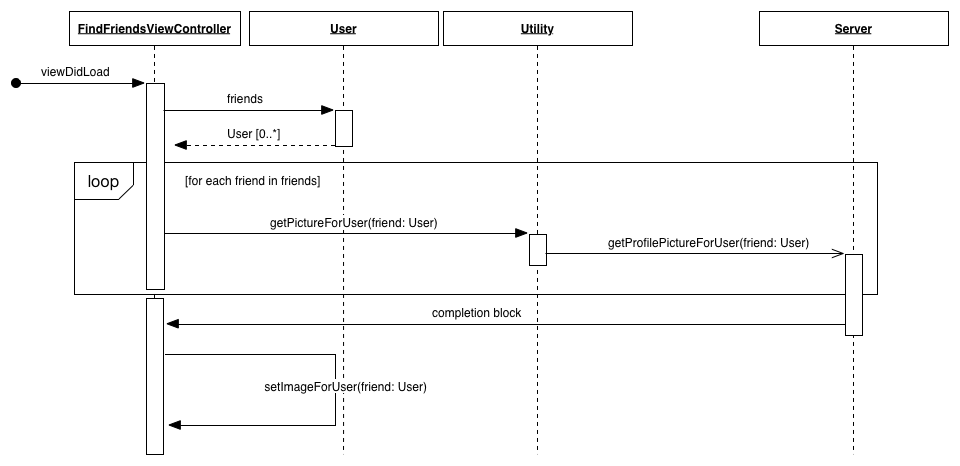
\includegraphics[width=\textwidth]{us15_sequence}
    \caption{FindFriendsViewController Sequence Diagram}
    \label{fig:us15_sequence}
\end{figure}
